\documentclass[../mainfile.tex]{subfiles}


\begin{document}

\section{The weak and strong Markov properties for Brownian Motion and first consequences}
\subsection{The weak Markov property}
In what follows, $B$ will denote a real-valued Brownian motion  in dimension $1$, but the statements will also hold in higher dimensions. 
\begin{defn}For every $t \geq 0$ we denote by $\mathcal{F}_t$ the $\sigma$-algebra generated by the random variables $\{B_r : 0 \leq r \leq t \}$. The Brownian filtration $( \mathcal{F}_t)_{t \geq 0}$ is then just the collection of these $\sigma$-fields (in particular we have $\mathcal{F}_t \subset \mathcal{F}_{t+h}$ for all $t,h \geq 0$). Moreover, for each finite time $T \geq 0$, we define the process $B^{(T)}=(B_t^{(T)})_{t \geq 0 }$ by \begin{align*}
B_t^{(T)}:= B_{T+t}-B_T.
\end{align*}
\end{defn}
The definition of Brownian motion (stationary independent increments) ensures immediately that:
\begin{lem}[Weak Markov property] When $T$ is a fixed, deterministic time, then $B^{(T)}$ is a Brownian motion that is independent of $\mathcal{F}_T$. 
\end{lem}
\subsubsection{Blumenthal's $0-1$ Law and consequences}
We also define for each $t \geq 0$, the $\sigma$-Field 
\begin{align*}
\mathcal{F}_{t+} := \bigcap_{h >0} \mathcal{F}_{t+h}, 
\end{align*}
which seems to contain some additional infinitesimal look into the future. 
\begin{rem} We can also think about the use of the above defined $\sigma$-field if we consider for instance a local maximum on $[0,t]$, for example a world record, and we wonder if our world record lasts at least for an infinitesimal time into the future $[0, t+h]$. 
\end{rem}
\newpage
\begin{prop}[Blumenthal's $0-1$ law] For the Brownian filtration, the $\sigma$-field $\mathcal{F}_{0+}$ is trivial in the sense that for all events $A \in \mathcal{F}_{0+}$ we have either $\mathbb{P}(A)=0$ or $\mathbb{P}(A)=1$. 
\end{prop}
\begin{proof}
Let us take $A \in \mathcal{F}_{0+}$, we then have for all $h>0$ also that $A \in \mathcal{F}_h$. Let us prove that $A$ is necessarily independent of $(B_{t_1}, \dots , B_{t_p})$ for all fixed times $0 < t_1< \dots < t_p$. Recall that for this, it is enough to prove that for any bounded continuous function $f: \mathbb{R}^p \to \mathbb{R}$ we have
\begin{align*}
\mathbb{E}(1_A f(B_{t_1},  \dots , B_{t_p}) = \mathbb{P}(A) \mathbb{E}(f (B_{t_1}, \dots , B_{t_p})).
\end{align*}
Let $h>0$. By dominated convergence and the continuity of $B$ we easily establish that 
\begin{align*}
\mathbb{E}(1_A f(B_{t_1},  \dots , B_{t_p})) = \lim_{h \to 0} \mathbb{E}(1_A f(B_{t_1+h}-B_h, \dots ,  B_{t_p+h}-B_h)) \\
= \lim_{h \to 0} \mathbb{E}(\overbrace{1_A}^{\in \mathcal{F}_h} f(\underbrace{B_{t_1}^{(h)}, \dots , B_{t_p}^{(h)})}_{\text{indep. of } \mathcal{F}_h}) \overset{\text{M.P.}}= \lim_{h \to 0} \mathbb{P}(A) \mathbb{E}(f(B_{t_1}^{(h)} , \dots , B_{t_p}^{(h)})) \\
= \mathbb{P}(A) \mathbb{E}(f(B_{t_1}, \dots , B_{t_p}))
\end{align*}
By a monotone class argument this establishes that $A$ is independent of $\mathcal{F}_\infty$, but then since $A \in \mathcal{F}_h \subset \mathcal{F}_\infty$ we conclude that $A$ is independent of itself, in particular we have
\begin{align*}
\mathbb{P}(A)= \mathbb{P}(A \cap A) = \mathbb{P}(A)^2 \implies \mathbb{P}(A) = 0 \text{ or } 1. 
\end{align*}
\end{proof}
Here is a nice and easy consequence of Blumenthal's $0-1$ law. 
\begin{prop} Almost surely,
\begin{align*}
\limsup_{t \to 0 } \frac{B_t}{\sqrt{t}} = \infty \text{ and } \liminf_{t \to 0} \frac{B_t}{\sqrt{t}}= - \infty. 
\end{align*}
\end{prop}
\begin{rem} Note that this implies in particular that for all $\epsilon >0$, there exists infinitely many times $t \in (0 , \epsilon)$ at which $B_t=0$. Moreover, the Proposition implies that almost surely, Brownian motion is not Hölder continuous with exponent $1/2$ (nor with any exponent greater than $1/2$) and thus Brownian motion is, as expected, nowhere differentiable.
\\\\
In order to see the second remark, let $0 \leq s < t$ be arbitrary, we then have almost surely
\begin{align*}
\limsup_{t \to 0} \frac{B_t}{\sqrt{t}}=\infty = \limsup_{t \to s} \frac{B_{t-s}}{\sqrt{t-s}} =  \limsup_{t \to s} \frac{B_t-B_s}{\sqrt{t-s}}
\end{align*}
in particular we cannot have $|B_t-B_s| \leq C\sqrt{t-s}$ for some $C \in \mathbb{R}_{>0}$.
\end{rem}
\newpage
\begin{proof}
We define for each $\epsilon >0$, the random variable 
\begin{align*}
V_\epsilon := \sup_{ s \in (0, \epsilon]} \frac{B_s}{\sqrt{s}}.
\end{align*}
Thanks to the continuity of Brownian motion we can write $V_\epsilon = \sup \{ B_s/\sqrt{s} : s \in (0, \epsilon] \cap \mathbb{Q}\}$, and we notice that $V_\epsilon$ is $\mathcal{F}_\epsilon$ measurable. Moreover, obviously $t \mapsto V_t$ is increasing and thus we can define 
\begin{align*}
V_{0+}:= \lim_{ \epsilon \to 0} V_{\epsilon} = \inf_{ \epsilon >0 } V_\epsilon.
\end{align*}
So we see that the random variable $V_{0+}$ is $\mathcal{F}_\epsilon$-measurable for all $\epsilon >0$ and therefore $\mathcal{F}_{0+}$ measurable. Hence, by Blumenthal's $0-1$ law, we have that it is constant either $0$ or $1$. \\
\\
Recall that the scaling property of a Brownian motion tells us that for all $a>0$ we have $\frac{1}{a}B_{a^2t}$ is also a Brownian motion, in particular $\frac{1}{a}B_{a^2 t} \sim B_t$. We note by applying this scaling property,  that the law of $V_\epsilon$ does in fact not depend on $\epsilon$. Indeed, let us fix $M \geq 1$ integer, then we have almost surely 
\begin{align*}
\left\{ \sup_{s \in (0, \epsilon]} \frac{B_s}{\sqrt{s}} \geq M \right\} \overset{t:=s/\epsilon}= \left\{ \sup_{t \in (0, 1]} \frac{B_{\epsilon t}}{\sqrt{\epsilon t}} \geq M \right\} = \left\{ \sup_{t \in (0,1]} \frac{\frac{1}{\sqrt{\epsilon}} B_{\epsilon t}}{\sqrt{t}} \geq M \right\} \\
= \left\{ \sup_{t \in (0,1]} \frac{B_t}{\sqrt{t}} \geq M \right\}
\end{align*}
Where in the last step the scaling property with $a= \sqrt{\epsilon}$ was used. So we have shown that $\mathbb{P}(V_\epsilon \geq M)= \mathbb{P}(V_1 \geq M)$, thus we finally get, \begin{align*}
\mathbb{P}(V_{0+} \geq M ) = \lim_{ \epsilon \to 0} \mathbb{P}(V_\epsilon \geq M ) = \mathbb{P}(V_1 \geq M )  = \mathbb{P} \left( \sup_{t \in (0,1]} \frac{B_t}{\sqrt{t}} \geq M \right) \\
\geq \mathbb{P}(\sup_{t \in (0,1]} B_t \geq M ) \geq \mathbb{P}( B_1 \geq M ) >0.
\end{align*}
So by Blumenthal's $0-1$ law we get that for all $M \in \mathbb{N}_{ \geq 1}$, $\mathbb{P}(V_{0+} \geq M ) = 1$. Thus we can exchange almost surely with for all $M$ integer to get 
\begin{align*}
\mathbb{P}( \forall M \geq 1, V_{0+} \geq M )=1,
\end{align*}
i.e. $V_{0+} = \infty$ almost surely. We can apply this also to the Brownian motion $-B$, to get the second statement. 
\end{proof}
\newpage
\subsection{Stopping times and the strong Markov property}
The goal of this section is to extend the weak Markov property to the case where $T$ is replaced by special random times.
\begin{defn} A random variable $T \in \mathbb{R}_+ \cup \{ \infty\}$ is a stopping time for a filtration $( \mathcal{F}_t)_{t \geq 0}$ if for every $t \geq 0$, the event $ \{T \leq t \}$ is in $\mathcal{F}_t$. We also define the $\sigma$-field of the past before $T$ as 
\begin{align*}
\mathcal{F}_T := \{ A \in \mathcal{F}_\infty : \forall t \geq 0, A \cap \{T \leq t \} \in \mathcal{F}_t \}.
\end{align*}
It intuitively corresponds to all the information (about everything) that has happened up to random time $T$. 
\end{defn}
\begin{rem} A good intuitive way to think about the definition of stopping times is that when $T$ has occurred, then one actually knows it. Here is a neat example to have in mind of a stopping time: You're driving on the highway, when a red car passes you, you take the next exit. Here is an example of a non-stopping time: One year before the next big earthquake. 
\end{rem}
\begin{prop}[Strong Markov property] Let $T$ be a stopping time (with respect to the Brownian filtration) such that $T< \infty$ almost surely. Then the process $B^{(T)} := (B_t^{(T)}=B_{T+t}-B_T)_{t \geq 0}$ is a Brownian motion independent of $\mathcal{F}_T$. 
\end{prop}
\begin{figure}[hbtp]
\centering
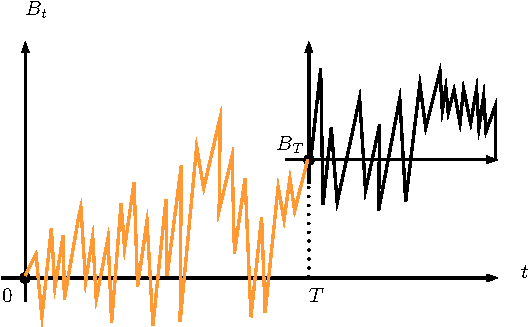
\includegraphics[scale=.932]{markovprop.pdf}
\caption{Qualitative picture of the strong Markov property. If we "reboot" the Brownian Motion at random stopping time $T$ (notice the shift of axis, $B^{(T)}$ starts at $0$), then what we observe is again a Brownian motion that is independent of its past $\mathcal{F}_T$ (orange).}
\end{figure}
\newpage
\begin{proof}
Let $A \in \mathcal{F}_T$, we want to prove that for all $t_1 < \dots < t_p$ the event $A$ is independent of $(B_{t_1}^{(T)}, \dots , B_{t_p}^{(T)})$ and that $(B_{t_1}^{(T)}, \dots , B_{t_p}^{(T)})$ has the same law as $(B_{t_1}, \dots , B_{t_p})$. In order to prove these two statements, it is enough to check that for all $f: \mathbb{R}^p \to \mathbb{R}$ continuous and bounded, we have 
\begin{align*}
\mathbb{E}(1_A f(B_{t_1}^{(T)}, \dots , B_{t_p}^{(T)})) = \mathbb{P}(A) \mathbb{E}(f(B_{t_1}^{(T)}, \dots ,  B_{t_p}^{(T)})),
\end{align*}
and
\begin{align*}
\mathbb{E}(f(B_{t_1}^{(T)}, \dots , B_{t_p}^{(T)})) = \mathbb{E}(f(B_{t_1},  \dots , B_{t_p}))
\end{align*}
We work with the discrete approximation of the stopping $T$. I.e. we define $T_n$ to be the smallest multiple of $2^{-n}$ such that $T \leq T_n$ ($T_n=$ smallest $j2^{-n}$ with $j2^{-n} \geq T)$. It is then an easy exercise to see that $T_n$ are also a stopping times w.r.t. the Brownian filtration and that $\{T_n=j2^{-n}\} \in \mathcal{F}_{j2^{-n}}$. \\
\\
We then define for each given $n$, $A_j= A \cap \{T_n= j2^{-n}\}.$ Then, each $A_j$ is in $\mathcal{F}_{j2^{-n}}$ and $A= \cup_j A_j$ as a disjoint union of the $A_j$'s. So we get:
\begin{align*}
\mathbb{E}(1_A f(B_{t_1}^{(T_n)}, \dots , B_{t_p}^{(T_n)}))= \sum_{j=0}^\infty \mathbb{E}(1_{A_j} f(B_{t_1}^{(T_n)}, \dots , B_{t_p}^{(T_n)})) \\
= \sum_{j=0}^\infty \mathbb{E}(1_{A_j} f(B_{t_1}^{(j2^{-n})}, \dots , B_{t_p}^{(j2^{-n})})) \overset{\text{W.M.P.}}= \sum_{j=0}^\infty \mathbb{P}(A_j) \mathbb{E}(f(B_{t_1}^{(j2^{-n})}, \dots , B_{t_p}^{(j2^{-n})})) \\
= \sum_{j=0}^\infty \mathbb{P}(A_j) \mathbb{E}(f(B_{t_1}, \dots , B_{t_p})) = \mathbb{P}(A) \mathbb{E}(f(B_{t_1}, \dots , B_{t_p}))
\end{align*}
But by dominated convergence and the continuity of Brownian motion we also have $\mathbb{E}(1_A f(B_{t_1}^{(T_n)}, \dots , B_{t_p}^{(T_n)})) \to \mathbb{E}(1_A f(B_{t_1}^{(T)}, \dots , B_{t_p}^{(T)}))$ as $n \to \infty$ almost surely. So finally we get \begin{align*}
\mathbb{E}(1_A f(B_{t_1}^{(T)}, \dots , B_{t_p}^{(T)})) = \mathbb{P}(A) \mathbb{E}(f(B_{t_1}, \dots , B_{t_p})).
\end{align*}
\end{proof}
\begin{rem} An equivalent way of phrasing the strong Markov property will be that (under the same conditions, $T$ being a finite stopping time) for all $f: \mathbb{R}^{\times \mathbb{R}_+} \to \mathbb{R}$ bounded and continuous (measurable would be enough) we have for all $x \in \mathbb{R}$, 
\begin{align*}
\mathbb{E}_x[f((B_{T+t})_{t \geq 0}) \mid \mathcal{F}_T] = \mathbb{E}_{B_T} [f((B_t)_{t \geq 0})]
\end{align*}
i.e. conditionally on $\mathcal{F}_T$ the process $(B_{T+t})_{t \geq 0}$ is again a Brownian motion, it is independent of $\mathcal{F}_T$ and has the same law as $B$ started from $B_T$.
\end{rem}

\newpage
\subsubsection{Reflection principle and consequences}
Suppose that $T$ is a stopping time for the Brownian filtration and assume that $T$ is almost surely finite. We now construct a new process $\tilde{B}$ as follows: for all $t \geq 0 $
\begin{align*}
\tilde{B}_t := \begin{cases} B_t, & t \leq T \\ 
B_T -(B_t-B_T), & t \geq T \end{cases}
\end{align*}
In other words, the increments of $\tilde{B}$ after the stopping time $T$ are the opposite of those of $B$.
\begin{figure}[hbtp]
\centering
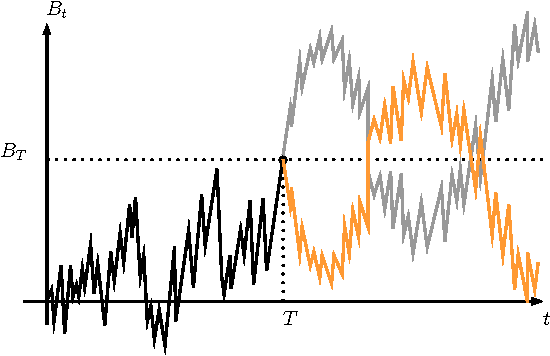
\includegraphics[scale=1]{reflectionprinc.pdf}
\caption{Depiction of the process $\tilde{B}$. We see the Brownian motion $B_t$ (black + grey) and the reflection after stopping time $T$ (depicted in orange) and the process $\tilde{B}$ (black + orange). }
\end{figure}
\begin{prop}[Reflection principle] The process $\tilde{B}$ is also a Brownian motion. 
\end{prop}
\begin{proof}
The strong Markov property says that the process $B^{(T)}$ is a Brownian motion and independent of $\mathcal{F}_T$. Hence, the process $-B^{(T)}$ is also a Brownian motion independent of $\mathcal{F}_T$. But we can reconstruct $B$ from the pair $(B_t, t \leq T)$ and $B^{(T)}=(B_{T+t}-B_T)_{t \geq 0 }$ in exactly the same way in which $\tilde{B}$ is reconstructed from the pair $(B_t, t \leq T)$ and $-B^{(T)}$, which implies that $B$ and $\tilde{B}$ have the same law. 
\end{proof}
\newpage
\begin{cor} Let $B$ be a Brownian motion in dimension $1$. For every $t>0$, define the \textit{running maximum} $S_t:= \max_{s \leq t} B_s$. For every $a \geq 0$ and $h \geq 0$ we have 
\begin{align*}
\mathbb{P}(S_t \geq a , B_t \leq a-h ) = \mathbb{P}(B_t \geq a+h).
\end{align*} 
Moreover, for each given $t$, the variable $S_t$ has the same distribution as $|B_t|$. 
\end{cor}
\begin{proof}
Let $T_a = \inf\{ t \geq 0 : B_t=a\}$. We know that (best seen in a picture) $\{S_t \geq a\} = \{T_a \leq t \}$. We obtain:
\begin{align*}
\mathbb{P}(S_t \geq a , B_t \leq a -h ) = \mathbb{P}(T_a \leq t, B_t-B_{T_a} \leq -h) = \mathbb{P}(T_a \leq t ,  B_{t-T_a}^{(T_a)} \leq -h) \\
\overset{1)}= \mathbb{P}(T_a \leq t, - \tilde{B}_{t-T_a}^{(T_a)} \leq -h ) = \mathbb{P}(T_a \leq t , \tilde{B}_{t-T_a}^{(T_a)} \geq h) = \mathbb{P}(T_a \leq t , \tilde{B}_{t}-\tilde{B}_{T_a} \geq h)  \\
\overset{2)}= \mathbb{P}(T_a \leq t, \tilde{B}_t - B_{T_a} \geq h ) = \mathbb{P}(T_a \leq t, \tilde{B}_t \geq a+h) \overset{\text{R.P.}}= \mathbb{P}(T_a \leq t,B_t \geq a+h)  \\
\overset{3)}= \mathbb{P}(B_t \geq a+h).
\end{align*} 
Where we used: 
\begin{enumerate}
\item It is easily seen that on $t \geq T_a$ we have $\tilde{B}_{t-T_a}^{(T_a)} = \tilde{B}_{t}-\tilde{B}_{T_a} \overset{\text{def}}=  B_{T_a}-(B_t-B_{T_a})-a = B_{T_a}-B_t$. Geometrically this is obvious when we look at the previous figure. 
\item By definition, as already used in 1. above, we have $\tilde{B}_{T_a}=B_{T_a}=a$. 
\item We have $\{B_t \geq a +h \} \subset \{ T_a \leq t\}$, indeed if for some fixed $t \geq 0$ we have $B_t \geq a+h$ then necessarily the first time when $B_t$ meets the height $a$ must occur before time $t$, i.e. $T_a \leq t$. 
\end{enumerate}
And R.P. stands for Reflection Principle. 
\\\\
To establish the second claim we choose $h=0$ to see that 
\begin{align*}
\mathbb{P}(S_t \geq a) = \mathbb{P}(S_t \geq a , B_t \leq a) + \mathbb{P}(S_t \geq a , B_t \geq a) \\ \overset{h=0}= \mathbb{P}(B_t \geq a) + \mathbb{P}(S_t  \geq a, B_t \geq a) = 2 \mathbb{P}(B_t \geq a) = \mathbb{P}(|B_t|  \geq a). 
\end{align*}
Where obviously $\{B_t \geq a \} \subset \{ S_t \geq a \}.$
\end{proof}
\newpage
\subsubsection{The zero-set of a Brownian motion}
We now state and prove another property of a Brownian motion which just further illustrates that a Brownian motion is quite a strange continuous curve. Let us define the zero-set of a Brownian motion as 
\begin{align*}
\mathcal{Z}:= \{ t \geq 0 : B_t = 0 \}. 
\end{align*}
\begin{prop} Almost surely, the set $\mathcal{Z}$ is a perfect set (i.e. it is an non-empty closed set with no isolated points).
\end{prop}
\begin{rem} \
\begin{enumerate}
\item Recall that a point $t \in Z$ is called isolated by definition if for all $\epsilon >0$ we have $Z \cap ( (t- \epsilon, t+ \epsilon) \setminus \{t\}) \neq \emptyset$.
\item It is an elementary exercise to show that a non-empty closed subset of $\mathbb{R}$ with no isolated points has the same cardinality as $\mathbb{R}$. 
\end{enumerate} 
\end{rem}
\begin{proof}
The set $\mathcal{Z}$ is closed almost surely thanks to the continuity of $B$. \textit{(A subset $D$ of a metric space is closed iff it contains all limits of seq. in $D$)}. \\\\
For $q \in \mathbb{Q}_+(= \mathbb{Q} \cap \mathbb{R}_+)$ we define the stopping time $\tau_q = \inf \{ t \geq q : B_t=0 \}$. Clearly if we take $T \in \mathcal{Z}$ (i.e. $B_T=0)$ and if we assume that $T$ is isolated from the left (i.e. $\exists \epsilon >0$ such that $(T- \epsilon , T) \cap \mathcal{Z} = \emptyset)$ then $\exists q \in \mathbb{Q}_+$ such that $\tau_q=T$. \\
\\
On the other hand, we know that for all such $q$,  $B^{(\tau_q)}$ is distributed like a Brownian motion, and we have seen ($\limsup_{t \to 0} B_t/\sqrt{t}=\infty)$ that almost surely $B^{( \tau_q)}$ has infinitely many zeros in any interval $(0, \epsilon)$, in particular $\tau_q$ is not isolated from the right in $\mathcal{Z}$. \\
\\
Consequently,  we have almost surely for all $q \in \mathbb{Q}_+$, that $\tau_q$ is not isolated in $\mathcal{Z}$ from the right. But then almost surely for all $t \in \mathcal{Z}$ which are isolated from the left we have 
\begin{align*}
t \in \bigcup_{q  \in \mathbb{Q}} \{\tau_q\},
\end{align*}
so $t$ is not isolated from the right and therefore $\mathcal{Z}$ has no isolated points. 
\end{proof}
\begin{rem} The Lebesgue measure $\lambda ( \mathcal{Z})$ of $\mathcal{Z}$ is almost surely equal to zero, indeed, by Fubini's theorem
\begin{align*}
\mathbb{E}( \lambda ( \mathcal{Z})) = \mathbb{E} \left( \int_0^\infty 1_{B_t=0} dt \right) = \int_0^\infty \mathbb{P}(B_t=0)dt =0
\end{align*}
which entails that $\lambda( \mathcal{Z})=0$ almost surely. 
\end{rem}
\newpage
\subsection{Analogous results for multidimensional Brownian motion}
Let us briefly list which results in the previous section can be immediately generalized to the case where one considers a Brownian motion $B$ in $d$-dimensional space with $d \geq 2$ instead of $d=1$.
\begin{itemize}
\item The weak Markov property.
\item The strong Markov property.
\item Blumenthal's $0-1$ law. 
\end{itemize}
The statements and proofs are exactly the same as in the one-dimensional case. 
\subsubsection{One extension of some $1$D results/ideas}
We start with an application of Blumenthal's $0-1$ law in higher dimensions. Let $(B_t)_{t \geq 0}$ be a Brownian motion in $\mathbb{R}^d, d \geq 2$, started at the origin $0$. Let $\mathcal{C}$ be an open subset of $\mathbb{R}^d \setminus \{0\}$ such for some fixed $r>0$, it contains a union of balls $\mathcal{B}(x_n,r|x_n|)$, where $x_n$ is some sequence in $\mathbb{R}^d \setminus \{0\}$ with $x_n \to 0$ (we can always assume that $|x_n|$ decreasing with $n$). That is, $\exists r>0$ and there exists a sequence $x_n \to 0$ in $\mathbb{R}^d \setminus \{0\}$ such that 
\begin{align*}
\bigcup_{n \in \mathbb{N}} \mathcal{B}(x_n,r|x_n|) \subset \mathcal{C}. 
\end{align*}
A good example to have in mind of such a set if when $\mathcal{C}$ is a cone with apex at $0$. 
\begin{figure}[hbtp]
\centering
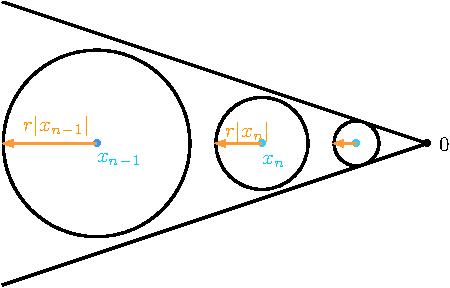
\includegraphics[scale=1]{cone.pdf}
\caption{$\mathcal{C}$ is a cone with apex at $0$.}
\end{figure}
\newpage
\begin{prop} Almost surely, for all $\epsilon >0$ there exists $t \in (0, \epsilon)$ such that $B_t \in \mathcal{C}$. 
\end{prop}
\begin{proof}
Let us define for $n_0 \in \mathbb{N}$ 
\begin{align*}
V_{n_0} := \bigcup_{n \geq n_0} \{ B_{|x_n|^2} \in \mathcal{B}(x_n, r|x_n|) \rbrace.
\end{align*}
Then $V_{n_0}$ is measurable with respect to
\begin{align*}
\mathcal{F}_{ \max_{n \geq n_0}|x_n|^2}. 
\end{align*}
We have
\begin{align*}
V_\infty := \bigcap_{n_0 \geq 0} V_{n_0} = \{ \exists \text{ infinitely many } n's : B_{|x_n|^2} \in \mathcal{B}(x_n,r|x_n|) \rbrace.
\end{align*}
Since also $V_{n_0+1} \subset V_{n_0}$ we have for all $\tilde{n}$ that 
\begin{align*}
V_\infty = \bigcap_{n_0 > \tilde{n}} V_{n_0},
\end{align*}
in particular $V_\infty$ is in $F_{0+}$ and therefore we have thanks to Blumenthal's $0-1$ law that $\mathbb{P}(V_\infty)=0$ or $1$. We want to show that this probability is $1$. 

\begin{align*}
\mathbb{P}(V_\infty)&= \lim_{n_0 \to \infty} \mathbb{P}(V_{n_0}) \geq \lim_{n_0 \to \infty} \mathbb{P}( B_{|x_{n_0}|^2} \in \mathcal{B}( x_{n_0},  r|x_{n_0}| )  \\ &= \lim_{n_0 \to \infty} \mathbb{P} \left[ \frac{1}{|x_{n_0}|} B_{|x_{n_0}|^2}  \in \mathcal{B}\left( \frac{x_{n_0}}{|x_{n_0}|}, r \right) \right] \overset{1)}=  \lim_{n_0 \to \infty} \mathbb{P}(B_1 \in \mathcal{B}(x_{n_0}/|x_{n_0}| , r ) )  \\
&\overset{2)} = \lim_{n_0 \to \infty}\mathbb{P}(B_1 \in \mathcal{B}(1.,r)) = \mathbb{P}(B_1 \in \mathcal{B}(1.,r)) >0.
\end{align*}
Where we used:
\begin{enumerate}
\item the scaling invariance at time $t=1$ $\frac{1}{a}B_{a^2t} \sim B_t$.
\item The isotropy property of a Brownian motion,  it just states that for all linear isometries $\phi$ we have $\Phi(B)$ is still a BM in $\mathbb{R}^d$ and $1.=(1,0,0 \dots ,0)\in \mathbb{R}^d$. 
\end{enumerate}
\end{proof}
\end{document}